%%%%%%%%%%%%%%%%%%%%%%%%%%%%%%%%%%%%%%%%%
% Journal Article
% LaTeX Template
% Version 1.3 (9/9/13)
%
% This template has been downloaded from:
% http://www.LaTeXTemplates.com
%
% Original author:
% Frits Wenneker (http://www.howtotex.com)
%
% License:
% CC BY-NC-SA 3.0 (http://creativecommons.org/licenses/by-nc-sa/3.0/)
%
%%%%%%%%%%%%%%%%%%%%%%%%%%%%%%%%%%%%%%%%%

%----------------------------------------------------------------------------------------
%	PACKAGES AND OTHER DOCUMENT CONFIGURATIONS
%----------------------------------------------------------------------------------------

\documentclass[twoside]{article}

\usepackage{etex}

\usepackage{lipsum} % Package to generate dummy text throughout this template

\usepackage[sc]{mathpazo} % Use the Palatino font
\usepackage[T1]{fontenc} % Use 8-bit encoding that has 256 glyphs
\usepackage[utf8]{inputenc}
\linespread{1.05} % Line spacing - Palatino needs more space between lines
\usepackage{microtype} % Slightly tweak font spacing for aesthetics
\usepackage{amsmath}
\usepackage{listings}

\lstset{
  basicstyle=\small,
  breaklines=true
}

\usepackage[hmarginratio=1:1,top=32mm,columnsep=20pt]{geometry} % Document margins
\usepackage{multicol} % Used for the two-column layout of the document
\usepackage[hang, small,labelfont=bf,up,textfont=it,up]{caption} % Custom captions under/above floats in tables or figures
\usepackage{booktabs} % Horizontal rules in tables
\usepackage{float} % Required for tables and figures in the multi-column environment - they need to be placed in specific locations with the [H] (e.g. \begin{table}[H])
\usepackage{hyperref} % For hyperlinks in the PDF
\usepackage{multirow}

\usepackage{syntax}
\setlength{\grammarparsep}{5pt plus 1pt minus 1pt} % increase separation between rules
\setlength{\grammarindent}{6em} % increase separation between LHS/RHS 

\usepackage{lettrine} % The lettrine is the first enlarged letter at the beginning of the text
\usepackage{paralist} % Used for the compactitem environment which makes bullet points with less space between them

\usepackage{abstract} % Allows abstract customization
\renewcommand{\abstractnamefont}{\normalfont\bfseries} % Set the "Abstract" text to bold
\renewcommand{\abstracttextfont}{\normalfont\small\itshape} % Set the abstract itself to small italic text

\usepackage{tikz}
\usetikzlibrary{shapes.multipart}

\newcommand{\rparen}{)}

\usepackage{titlesec} % Allows customization of titles
\renewcommand\thesection{\Roman{section}} % Roman numerals for the sections
\renewcommand{\thesubsection}{\thesection\hspace{1mm}\alph{subsection}}
\titleformat{\section}[block]{\large\scshape\centering}{\thesection}{1em}{} % Change the look of the section titles
\titleformat{\subsection}[block]{\large}{\thesubsection\rparen}{1em}{} % Change the look of the section titles

\usepackage{fancyhdr} % Headers and footers
\pagestyle{fancy} % All pages have headers and footers
\fancyhead{} % Blank out the default header
\fancyfoot{} % Blank out the default footer
\fancyhead[C]{TDT4205 Compilers $\bullet$ Assignment Five $\bullet$ \date{\today}} % Custom header text
\fancyfoot[RO,LE]{\thepage} % Custom footer text

%----------------------------------------------------------------------------------------
%	TITLE SECTION
%----------------------------------------------------------------------------------------

\title{\vspace{-15mm}\fontsize{24pt}{10pt}\selectfont\textbf{Theory for Assignment Five}} % Article title

\author{
    \large
    \textsc{Øyvind Robertsen} \\ % Your name
    \normalsize Norwegian University of Science \& Technology \\ % Your institution
    \normalsize \href{mailto:oyvinrob@stud.ntnu.no}{oyvinrob@stud.ntnu.no} % Your email address
    \vspace{-5mm}
}
\date{}

%----------------------------------------------------------------------------------------

\begin{document}

\maketitle % Insert title

\thispagestyle{fancy} % All pages have headers and footers

%----------------------------------------------------------------------------------------
%	ABSTRACT
%----------------------------------------------------------------------------------------

%\begin{abstract}

%\noindent \lipsum[1] % Dummy abstract text

%\end{abstract}

%----------------------------------------------------------------------------------------
%	ARTICLE CONTENTS
%----------------------------------------------------------------------------------------

\begin{multicols}{2} % Two-column layout throughout the main article text

    \section{Problem 1}

    Stack contents at first passing of position 1 is given in figure \ref{fig:prob1stack1}. The second time position 1 is reached, the stack also contains the entries in figure \ref{fig:prob1stack2}. In both figures, all \texttt{ret addr}-entries are the result of the callee pushing the LR contents onto the stack, and similarily for the \texttt{fp <whatever>}-entries.

    \begin{figure}[H]
        \centering
        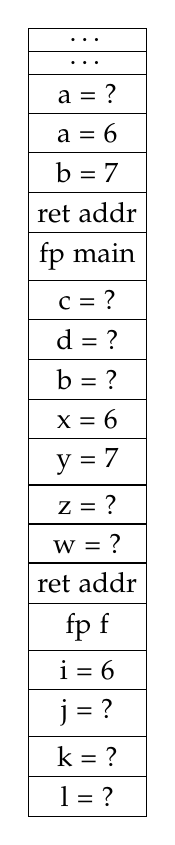
\begin{tikzpicture}[stack/.style={rectangle split, rectangle split parts=#1, draw, anchor=center}]
            \node[stack=20] {
            \nodepart{one}\ldots 
            \nodepart{two}\ldots
            \nodepart{three}a = ?
            \nodepart{four}a = 6
            \nodepart{five}b = 7
            \nodepart{six}ret addr
            \nodepart{seven}fp main
            \nodepart{eight}c = ?
            \nodepart{nine}d = ?
            \nodepart{ten}b = ?
            \nodepart{eleven}x = 6
            \nodepart{twelve}y = 7
            \nodepart{thirteen}z = ?
            \nodepart{fourteen}w = ?
            \nodepart{fifteen}ret addr
            \nodepart{sixteen}fp f
            \nodepart{seventeen}i = 6
            \nodepart{eighteen}j = ?
            \nodepart{nineteen}k = ?
            \nodepart{twenty}l = ?
            };
        \end{tikzpicture}
        \caption{Stack contents at first passing of position 1} \label{fig:prob1stack1}
    \end{figure}
    
    \begin{figure}[H]
        \centering
        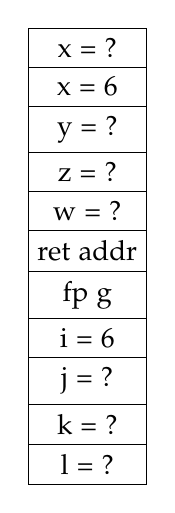
\begin{tikzpicture}[stack/.style={rectangle split, rectangle split parts=#1, draw, anchor=center}]
            \node[stack=11] {
            \nodepart{one}x = ?
            \nodepart{two}x = 6
            \nodepart{three}y = ?
            \nodepart{four}z = ?
            \nodepart{five}w = ?
            \nodepart{six}ret addr
            \nodepart{seven}fp g
            \nodepart{eight}i = 6
            \nodepart{nine}j = ?
            \nodepart{ten}k = ?
            \nodepart{eleven}l = ?
            };
        \end{tikzpicture}
        \caption{Additional stack contents at second passing of position 1} \label{fig:prob1stack2}
    \end{figure}

    \section{Problem 2}

    \begin{verbatim}
    f:
        push {lr, fp}
        mov fp, sp
        ldr r1, [fp, #12] // address of array
        ldr r2, [fp, #8] // Get b
        push { #0 } // INT C;
        mov r3, #5 // access offset
        mul r3, r3, #4 // offset * 4
        add r4, r1, r3 // baseaddress + offset * 4
        ldr r5, [r4] // a[5]
        str r5, [fp, #-4] // c = a[5]
        push {r1, r2, r3, r4, r5} // store registers
        push {r2, r1} // Push parameters
        bl g
        pop {r1, r2} // remove parameters
        pop {r5, r4, r3, r2, r1} // Restore registers
        mov sp, fp // return
        pop {fp, pc}

    g:
        push {lr, fp}
        mov fp, sp
        ldr r1, [fp, #12] // get x
        ldr r2, [fp, #8] // get y
        push { #0 } // INT d;
        str r1, [fp, #-4] // d = x;
        mul r3, r1, #4 // offset * 4
        add r4, r2, r3 // access address
        ldr r0, [r4] // y[d]
        mov sp, fp // return
        pop {fp, pc}
    \end{verbatim}

    \section{Problem 3}

    Since the stack grows "downward", from high address to low, while static arrays are organized with the first entry on the top of the stack, \texttt{array[6]} will refer to the stack entry where the link register value (the return address) is stored.
    As a result the return address of the \texttt{fill\_array}-function is overwritten with the address of the \texttt{never\_called}-function.
    When the return address is popped into the PC-register, execution is 

    \begin{figure}[H]
        \centering
        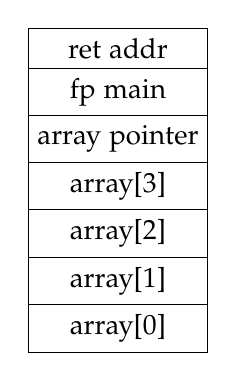
\begin{tikzpicture}[stack/.style={rectangle split, rectangle split parts=#1, draw, anchor=center}]
            \node[stack=7] {
            \nodepart{one}ret addr
            \nodepart{two}fp main
            \nodepart{three}array pointer
            \nodepart{four}array[3]
            \nodepart{five}array[2]
            \nodepart{six}array[1]
            \nodepart{seven}array[0]
            };
        \end{tikzpicture}
        \caption{Relevant part of the stack for problem 3} \label{fig:prob3stack}
    \end{figure}

    \section{Problem 4}

    With a high-level IR, we remain close to the source language constructs and use a structure very similar to the AST. 
    Aforementioned tree-structure makes it convenient to perform transformations like moving around and copying subtrees.
    These are operations that would be very impractical to perform with a lower-level IR, as the sequence of instructions lacks the organization inherent of a tree structure.
    Therefore, function inlining and function cloning are optimizations commonly performed at this stage.

    Lower-level IR discards the tree structure in favour of an instruction set describing an abstract machine.
    This captures lower-level machine features and allows for more specialized optimizations than high-level IR.
    Dead code elimination, loop invariant code motion, branch prediction/optimization and loop unrolling are examples of optimizations that are common to perform using a lower-level IR.
    Common for all these is that they involve analysing code that would span several distinct subtrees in an AST, and therefore are not aided by the tree structure of the higher-level IR.
    Lower-level IR are usually close to the target architecture, allowing us to perform some platform dependent optimizations.

\end{multicols}
\newpage

    \section{Problem 5}

    \subsection{Function inlining}

    Function inlining refers to replacing a function call with the actual body of that function. 
    This eliminates the overhead introduced by the function call protocol and can therefore reduce execution time.
    Programmers often write wrapper functions for simple calculations, in order to increase the readability/understandability of their code.
    The \texttt{polynomial}-function in this problem is a very good example of this.
    Function inlining is usually performed early in the optimization process, while we are still using a high level, tree-like IR.

    Example:
    \begin{figure}[h]
        \centering
        \begin{verbatim}
        ...
        p1[i] = polynomial(1, 0, 4*4*s*i, i) - sin(a);
        p2[i] = polynomial(3, 1, 4*4*s*i, i) - f;
        ...
        \end{verbatim}
    \end{figure}

    could be transformed into

    \begin{figure}[h]
        \centering
        \begin{verbatim}
        ...
        float r;
        float a = 1;
        float b = 0;
        float c = 4*4*s*i;
        float x = i;
        r = a*x*x + b*x + c;
        p1[i] = r - sin(a);
        a = 3;
        b = 1;
        r = a*x*x + b*x + c;
        p2[i] = r - f;
        \end{verbatim}
    \end{figure}

    \subsection{Function cloning}

    Function cloning refers to creating specialized version of a function, optimizing it for specific call cases.
    If a function performs expensive operations (multiplication, division) on a parameter, we can create clones of the function where we assume that parameter to be 1 or 0.
    In the function clone, we can eliminate all these operations, seeing as we know that multiplying/dividing by 1 doesn't effect the outcome of the operation.
    We then replace all calls to the original function where the parameter in question is set to 0 or 1 with calls to our optimized versions.
    This is also an execution time optimization, but comes at a cost of increased program size.
    
    Example:
    \begin{figure}[h!]
        \centering
        \begin{verbatim}
        float polynomial(float a, float b, float c, float x) {
            return a*x*x + b*x + c;
        }
        \end{verbatim}
    \end{figure}
    
    In the given example code the function above is called two times, as \texttt{polynomial(1, 0, 4*4*s*i, i)} and \texttt{polynomial(3, 1, 4*4*s*i, i)}.
    The first call has the b-parameter set to zero, so we replace it with a call to \texttt{polynomial2(1, 4*4*s*i,i)}, where \texttt{polynomial2} is defined as follows:

    \begin{figure}[h!]
        \centering
        \begin{verbatim}
        float polynomial2(float a, float c, float x) {
            return a*x*x + c;
        }
        \end{verbatim}
    \end{figure}
    
    \subsection{Constant folding}

    Given that all operands of an expression is known at compile time, we can evaluate the expression preemptively, saving us an operation at runtime.
    This type of optimization is called constant folding, and is typically performed at each step in the overall optimization/code generation process.
    This way, we ensure that expressions with constant operators generated by other translations/optimizations are folded as well.

    Example:

    \begin{figure}[h!]
        \centering
        \begin{verbatim}
        ...
        p1[i] = polynomial(1, 0, 4*4*s*i, i) - sin(a);
        ...
        \end{verbatim}
    \end{figure}

    In the call to the \texttt{polynomial} function, we can evaluate the \texttt{4*4} subexpression at compile time, saving us six multiplications in total. (Two for each iteration of the loop.)
    This gives us:

    \begin{figure}[h!]
        \centering
        \begin{verbatim}
        ...
        p1[i] = polynomial(1, 0, 16*s*i, i) - sin(a);
        ...
        \end{verbatim}
    \end{figure}

    \subsection{Constant propagation}

    If the value of a variable is known to be constant, we directly replace all usages of that variable with the value.
    This can create more situations in which we can apply constant folding, and therefore reduce execution time.

    Example:

    In the handed out code, the variables \texttt{a} and \texttt{s} are given constant values that don't change throughout the program. 
    We replace all occurrences of them with the corresponding values.

    \newpage

    \begin{figure}[h!]
        \centering
        \begin{verbatim}
        ...
        float f = sin(1.57)*2;
        p1[i] = 0;
        p2[i] = 0;
        p1[i] = polynomial(1, 0, 4*4*16*i, i) - sin(1.57);
        p2[i] = polynomial(3, 1, 4*4*16*i, i) - f;
        ...
        \end{verbatim}
    \end{figure}


    \subsection{Dead code elimination}

    If a statement has no observable effect, we can safely eliminate that statement.
    This directly impacts execution time, as we are eliminating useless instructions.

    Example:

    \begin{figure}[h!]
        \centering
        \begin{verbatim}
        ...
        p1[i] = 0;
        p2[i] = 0;
        ...
        \end{verbatim}
    \end{figure}

    The two statements above are useless in the context of the program, as they are overwritten directly after, and can therefore safely be removed.
    
    \subsection{Loop-invariant code motion}

    Loop-invariant code motion refers to moving statements/expression that don't change during the execution of the loop out of the loop.
    This reduces execution time.

    Example:

    \begin{figure}[h!]
        \centering
        \begin{verbatim}
        ...
        for (int i = 0; i < 3; i++) {
            float f = sin(1.57)*2;
            p1[i] = 0;
            p2[i] = 0;
            p1[i] = polynomial(1, 0, 4*4*16*i, i) - sin(1.57);
            p2[i] = polynomial(3, 1, 4*4*16*i, i) - f;
        }
        ...
        \end{verbatim}
    \end{figure}

    In the snippet above, the \texttt{float f = sin(1.57)*2;} statement can be moved above the loop, without any externally visible side-effects.
    This results in the following:

    \begin{figure}[h!]
        \centering
        \begin{verbatim}
        ...
        float f = sin(a)*2;
        for (int i = 0; i < 3; i++) {
            p1[i] = 0;
            p2[i] = 0;
            p1[i] = polynomial(1, 0, 4*4*s*i, i) - sin(a);
            p2[i] = polynomial(3, 1, 4*4*s*i, i) - f;
        }
        ...
        \end{verbatim}
    \end{figure}


    \newpage
    \subsection{Common sub-expression elimination}

    A program that evaluates the same expression several times can be optimized to reuse the resulting value.
    Since we reduce the number of instructions to be ran by the CPU, execution time is reduced.

    Example:

    \begin{figure}[h!]
        \centering
        \begin{verbatim}
        ...
        for (int i = 0; i < 3; i++) {
            float f = sin(a)*2;
            p1[i] = 0;
            p2[i] = 0;
            p1[i] = polynomial(1, 0, 4*4*s*i, i) - sin(a);
            p2[i] = polynomial(3, 1, 4*4*s*i, i) - f;
        }
        ...
        \end{verbatim}
    \end{figure}

    There snippet above allows for two cases of common sub-expression elimination; \texttt{sin(a)} and \texttt{4*4*s*i}.
    We optimize:

    \begin{figure}[h!]
        \centering
        \begin{verbatim}
        ...
        for (int i = 0; i < 3; i++) {
            float t1 = sin(a);
            float f = t1*2;
            p1[i] = 0;
            p2[i] = 0;
            int t2 = 4*4*s*i;
            p1[i] = polynomial(1, 0, t2, i) - t1;
            p2[i] = polynomial(3, 1, t2, i) - f;
        }
        ...
        \end{verbatim}
    \end{figure}


    \newpage
    \subsection{Strengt reduction}

    Multiplication and division is expensive, addition and subtraction is cheap.
    Strength reduction refers to replacing occurrences of expensive operations with cheap ones.
    This is especially effective in loops, and is commonly performed on induction variables (variables that are linearily dependent on the iteration number.)
    Strength reduction can reduce execution time.

    Example:

    \begin{figure}[h!]
        \centering
        \begin{verbatim}
        float polynomial(float a, float b, float c, float x) {
            return a*x*x + b*x + c;
        }
        ...
        for (int i = 0; i < 3; i++) {
            float f = sin(a)*2;
            p1[i] = 0;
            p2[i] = 0;
            int t1 = 256*i;
            p1[i] = polynomial(1, 0, t1, i) - sin(a);
            p2[i] = polynomial(3, 1, t1, i) - f;
        }
        ...
        \end{verbatim}
    \end{figure}

    In the snippet above, we can perform two cases of strength reduction. The first one is in the \texttt{polynomial} function.


    \begin{figure}[h!]
        \centering
        \begin{verbatim}
        float polynomial(float a, float b, float c, float x) {
            return a*(x + x) + b*x + c;
        }
        \end{verbatim}
    \end{figure}

    The second is in the \texttt{256*i} expression in the calls to the function. 
    Here I've mentally applied constant propagation, constant folding and common sub-expression elimination for simplicity.
    The result is as follows:

    \begin{figure}[h!]
        \centering
        \begin{verbatim}
        ...
        int t1 = -256;
        for (int i = 0; i < 3; i++) {
            float f = sin(a)*2;
            p1[i] = 0;
            p2[i] = 0;
            t1 = t1 + 256;
            p1[i] = polynomial(1, 0, t1, i) - sin(a);
            p2[i] = polynomial(3, 1, t1, i) - f;
        }
        ...
        \end{verbatim}
    \end{figure}

    \subsection{Loop unrolling}

    By partially or completely rewriting a loop as a repeated sequence of similar statements, we can reduce the number of branches and loop maintainance overhead.
    The result is a more efficient program, at the expense of larger program size.

    Example:

    \begin{figure}[h!]
        \centering
        \begin{verbatim}
        ...
        for (int i = 0; i < 3; i++) {
            printf("%f, %f\n", p1[i], p2[i]);
        }
        \end{verbatim}
    \end{figure}

    The snippet above can be complete unrolled, resulting in the following:

    \begin{figure}[h!]
        \centering
        \begin{verbatim}
        ...
        printf("%f, %f\n", p1[0], p2[0]);
        printf("%f, %f\n", p1[1], p2[1]);
        printf("%f, %f\n", p1[2], p2[2]);
        ...
        \end{verbatim}
    \end{figure}

\end{document}
